\documentclass[11pt,a4paper]{article}
\usepackage[margin=2.0cm,top=2.2cm,bottom=2.2cm]{geometry}
\usepackage{amsmath,amssymb}
\usepackage{enumitem}
\usepackage{booktabs}
\usepackage{graphicx}
\graphicspath{{../presentation/assets/}{./}}
\usepackage{float}
\usepackage{placeins}
\usepackage{xcolor}
\usepackage{caption}
\captionsetup{font=small,labelfont=bf}
\usepackage[colorlinks=true, linkcolor=blue!45!black, urlcolor=blue!45!black, citecolor=blue!45!black]{hyperref}
\usepackage{parskip}
\usepackage{fancyhdr}
\setlength{\headheight}{13.6pt}
\pagestyle{fancy}\fancyhf{}
\lhead{Computational Genomics 76553}\rhead{Hackathon}\cfoot{\thepage}
\renewcommand{\headrulewidth}{0.4pt}
\begin{document}
\noindent{\LARGE\bfseries Matched-source re-analysis of human MASLD snRNA-seq\\[1pt]
preserves hepatocyte transcriptional zonation}\par
\vspace{0.45em}
\noindent\textbf{Roee Tekoah}~(\href{mailto:roee.tekoah@mail.huji.ac.il}{roee.tekoah@mail.huji.ac.il})\quad\textbf{·}\quad\textbf{Shira Gelbstein}\par
\vspace{0.12em}
\noindent{\small\color{black!55}Computational Genomics 76553~~·~~Hebrew University of Jerusalem~~·~~Hackathon}\par
\vspace{0.45em}
\noindent\textcolor{black!40}{\rule{\textwidth}{0.7pt}}\par
\vspace{0.6em}

{\small\noindent\textbf{Abstract.~}\textbf{Question.} Gribben et al.\ report that hepatocytes progressively lose their porto-central \emph{zonation} across the metabolic-dysfunction-associated steatotic liver disease (MASLD) spectrum, and ultimately transdifferentiate toward a biliary (cholangiocyte) program. We asked whether the single-nucleus transcriptomic leg of the progressive de-zonation claim survives once the way the tissue was obtained is taken into account. \textbf{Confound.} In this cohort, disease stage is collinear with tissue acquisition: the F0--F4 disease spectrum is 16-gauge needle biopsy, whereas both endpoints --- ``healthy'' and ``end-stage'' --- are deceased-donor whole-organ cubes. The healthy$\to$end-stage axis is therefore also an organ-cube$\to$needle$\to$explant axis. \textbf{Method.} Working on raw RNA UMI counts (not the shipped SCT matrix), with the donor as the unit of inference ($\sim$47 donors, 69{,}426 hepatocyte nuclei), we restricted the disease axis to the acquisition-matched needle biopsies (38 donors, fibrosis F1$\to$cirrhotic F4) and classified each hepatocyte by strict, mutually exclusive zonation anchors at an ambient-robust $\ge$2-UMI threshold on depth-normalized counts. We then ran a genome-wide donor-level pseudobulk differential-expression (DGE) scan (edgeR) to ask what else changes. \textbf{Matched-biopsy result.} Across the matched biopsy axis, hepatocyte transcriptional zonation is preserved: the pericentral-anchor fraction is flat/non-monotone (36/19/23/22/21\% for F0--F4), an ambient-robust equivalence test excludes a large coordinated shift ($\sim$20 percentage points) but not a subtle $\le$10-point drift, and the result is robust across the full sensitivity grid. \textbf{DGE result.} Of $\sim$21{,}000 tested genes, 64 reach FDR$<$0.05 at F4-vs-F1 and they are a biliary/ductular marker burden (EPCAM, GRHL2, SPINT2, SOX4, SOX9, B3GNT3) plus CXCL10; zonation genes are flat (GLUL FDR 0.80). \textbf{Conclusion.} In acquisition-matched MASLD biopsy tissue, the transcriptional evidence for progressive hepatocyte de-zonation does not appear; the one biopsy-stage change is a biliary-marker burden inside hepatocyte-labeled pseudobulk that is most consistent with cholangiocyte ambient RNA plus rare mixed/doublet nuclei --- a lead, not a closed result. We correct only the snRNA transcriptional leg; the paper's imaging, protein and organoid evidence are not addressed.}\par\vspace{0.5em}

\setcounter{tocdepth}{2}
\begingroup\renewcommand{\contentsname}{\normalsize Contents}{\small\tableofcontents}\endgroup
\vspace{0.6em}

\noindent\textit{Supplementary report (optional).} The required deliverable for this project is the presentation; this document is a complete written companion to it.

\vspace{0.4em}
\begin{table}[h]
\centering\small
\begin{tabular}{ll}
\toprule
\textbf{Course} & Computational Genomics 76553 -- Hackathon \emph{(placeholder; confirm course code/section)} \\
\textbf{Date} & 2026-06-23 \\
\textbf{Dataset} & Gribben et al., \emph{Nature} 2024, ``Acquisition of epithelial plasticity in \\
 & human chronic liver disease'' --- GSE202379 (single-nucleus RNA-seq component only) \\
\bottomrule
\end{tabular}
\end{table}

\section{Introduction}

\subsection{Hepatocyte zonation and epithelial plasticity}

The liver's repeating functional unit, the lobule, carries a steep chemical gradient: blood enters at the portal triads, relatively oxygen- and nutrient-rich, and flows inward to the central vein, where oxygen is depleted. Because a hepatocyte's environment depends on where it sits along this porto-central axis, hepatocytes specialise smoothly along it --- a division of labour called \textbf{zonation}. Broadly, the \textbf{periportal} pole runs much of the urea cycle (ASS1) and gluconeogenesis (PCK1, ALDOB), while the \textbf{pericentral} pole runs glutamine synthesis (GLUL) and cytochrome-P450 xenobiotic metabolism (CYP3A4, CYP2E1), maintained by an oxygen and Wnt/R-spondin gradient emanating from central-vein endothelium. Zonation is \emph{intra}-hepatocyte variation --- a question of \emph{where on the axis} a hepatocyte sits.

This must be kept distinct from \textbf{epithelial plasticity}, which is variation \emph{between} cell types: the normally locked boundary between hepatocyte (ALB) and cholangiocyte/biliary (KRT7, KRT19, SOX9) identity blurring to produce biphenotypic cells. De-zonation is a hepatocyte forgetting its \emph{address}; plasticity is a hepatocyte drifting away from \emph{being a hepatocyte}. The two phenomena are measured with separate gene sets and must not be conflated.

\subsection{The paper and the motivation}

Gribben et al.\ (\emph{Nature} 2024) profiled 47 liver samples by snRNA-seq across the MASLD spectrum (healthy, NAFLD/MASLD, MASH, cirrhosis, end-stage), yielding $\sim$99{,}809 QC-passing nuclei including 69{,}426 hepatocytes. Their headline biology is hepatocyte$\to$cholangiocyte transdifferentiation driven by PI3K-AKT-mTOR, supported by organoid and imaging evidence; as a secondary observation they report that hepatocytes progressively lose zonation, evidenced in the snRNA data by a pericentral-vs-periportal marker correlation (with a Welch's-$t$ comparison) pooled across donors and by a stage-split hepatocyte embedding. It is a careful, high-quality study, and the de-zonation reading is intuitive. The motivation here is narrow and specific: the snRNA de-zonation statistic pools the entire cohort across a sampling discontinuity, and we wanted to know whether the transcriptional signal survives when that discontinuity is removed.

\subsection{Research question}

\begin{itemize}[leftmargin=1.4em]
  \item \textbf{Primary.} Across an \emph{acquisition-matched} MASLD axis (needle-biopsy fibrosis F1$\to$cirrhotic F4), is hepatocyte transcriptional zonation preserved, or does it progressively collapse as the paper reports?
  \item \textbf{Secondary.} Given preserved zonal structure, what \emph{else} changes genome-wide in the hepatocyte transcriptome across the matched disease axis --- and what is the source of any such change?
\end{itemize}

\subsection{Hypothesis and operational goals}

The original project was framed around three hypotheses (H1: a de-zonation score rises monotonically with stage; H2: zone-specific programs --- e.g.\ pericentral CYP detox --- collapse earlier/faster; H3: the most de-zonated hepatocytes are the ones gaining biliary identity). Our operational goals reframe these into testable count-based endpoints that survive the confound: (i) quantify the tissue-acquisition confound directly; (ii) replace the relative, depth-sensitive marker-correlation ``ruler'' with a mechanism-resolving anchor classification on raw counts; (iii) bound how large a zonation shift the matched axis could have hidden; and (iv) run an honest genome-wide discovery scan for any other hepatocyte program.

\textbf{Thesis.} The transcriptomic evidence for \emph{progressive} hepatocyte de-zonation in this cohort is largely an artifact of tissue acquisition: the dramatic signal lives in deceased-donor organ tissue (healthy and end-stage), which is procured differently from the needle biopsies that make up the disease spectrum. Once the disease axis is restricted to acquisition-matched needle biopsies, hepatocyte transcriptional zonation is preserved against any large change, and the only genome-wide signal is a small biliary-marker burden whose origin is most consistent with compositional contamination (ambient cholangiocyte RNA and rare mixed/doublet nuclei) rather than widespread transdifferentiation --- though that source attribution is a lead, not a closed result. We correct only the single-nucleus transcriptional leg of the paper; its imaging, protein, organoid and spatial-architecture evidence are not addressed.

\section{Data and methods}

\subsection{Dataset and the matched axis}

The data are the snRNA-seq component of GSE202379: 47 donors, $\sim$99{,}809 QC-passing nuclei, 69{,}426 of them hepatocytes. From Paper 1's own Methods, tissue was obtained two different ways. The \textbf{disease spectrum} (38 donors, fibrosis F0--F4 $=$ 2/8/12/12/4 donors) came from \emph{16-gauge end-cut needle core biopsies} (``two ultrasound-guided needle core liver biopsies of approximately 2 cm''), right-lobe by construction. The \textbf{healthy} group (4 donors) and the \textbf{end-stage} group (5 donors) are \emph{deceased-donor whole-organ cubes} (``a cube of approximately 1 cm$^3$ was cut and frozen''), and for the explants (and two healthy donors) tissue was sampled from all three lobes (left, right, caudate). Our disease axis is therefore the \textbf{needle-biopsy donors only}.

A scoping note carried throughout: our ``biopsy F4'' (n$=$4) is \textbf{NASH-with-cirrhosis needle biopsies}, distinct from the 5 end-stage \emph{explant} donors, although both carry fibrosis score F4. The matched axis thus tests \emph{into established cirrhosis}, which is where de-zonation should be most visible if it occurs. F0 (n$=$2) is shown descriptively but is too thin to anchor inference; the inferential weight rests on F1--F4, with the best-powered interior at F1--F3 (n$=$8/12/12).

\subsection{Raw counts, not SCT}

The shipped expression matrix is an SCT (regularized-negative-binomial) model output, with depth squeezed to a synthetic budget --- appropriate for visualization but not for molecule-level questions such as co-detection of two markers in one nucleus or sensitivity to ambient RNA. All quantitative claims here are computed on the \textbf{raw RNA UMI counts} extracted from the RNA assay of the Seurat object, never on the SCT matrix.

\subsection{Depth normalization by binomial down-thinning}

Deeper-sequenced nuclei detect more genes for purely technical reasons, which would inflate any detection- or co-detection-based metric. To make detection fair across nuclei we \textbf{down-thin} each nucleus's raw UMIs to a common budget of \textbf{1{,}500 UMIs} by binomial thinning (nuclei below the budget are dropped), and average the resulting metrics over Monte-Carlo draws. The headline endpoints were re-checked at budgets of 1{,}000 / 1{,}500 / 3{,}000 UMIs; Monte-Carlo SD on donor-median fractions was 0.006--0.010.

\subsection{Procurement-stress module}

To quantify acute handling/dissociation stress we summed raw UMIs of an 8-gene module of immediate-early and heat-shock genes: \textbf{FOS, JUN, JUNB, JUND, ATF3, DUSP1, HSPA1A, HSPA1B}. A separate HIF/hypoxia panel (VEGFA, SLC2A1, LDHA, CA9, ENO1, PGK1) was held out as a \emph{contrast} to distinguish acute handling from chronic hypoxia. These are reported depth-matched, per nucleus, averaged across donors.

\subsection{Anchor classification (cell-state composition)}

Our central instrument --- which we call \textbf{anchor classification} (the field-standard name is differential cell-state composition; cf.\ miloR/scCODA/propeller) --- labels each hepatocyte by strict, mutually exclusive zonation markers on depth-normalized counts. \textbf{Pericentral (PC) anchors:} GLUL, CYP3A4. \textbf{Periportal (PP) anchors:} ASS1, PCK1, HAL, ALDOB. A nucleus is ``on-call'' for a pole if it carries \textbf{$\ge$2 UMI} (ambient-robust) of an anchor for that pole; it is then classed \textbf{PC}, \textbf{PP}, \textbf{dual} (on-call for both), or \textbf{null} (neither). The unit of inference is the \textbf{donor}; per-donor fractions are summarised by stage. We swept a sensitivity grid (GLUL-only / CYP3A4-only / both; $k$ in $\{1,2\}$; 2-of-4 / 3-of-4 on the PP side; ALDOB in/out; CPS1; strict-identity variants) and a marker-set ladder spanning 2 $\to$ 1{,}637 genes.

\subsection{Equivalence / bounding}

To turn the descriptive null into an affirmative statement we ran a two-one-sided-test (TOST) equivalence analysis on donor-level anchor fractions across F1-vs-F4 (n$=$8 vs 4) and the better-powered interior F1-vs-F3 (n$=$8 vs 12), reporting the 90\% confidence interval on the difference.

\subsection{Pseudobulk differential expression}

For ``what else changes,'' we summed each biopsy donor's hepatocyte raw UMIs into one count profile (\textbf{donor-level pseudobulk}, the recommended guard against pseudoreplication; Squair et al.\ 2021) and ran \textbf{edgeR}: \texttt{filterByExpr} against the design ($\to$ 21{,}022 genes retained), TMM normalization (which corrects depth \emph{and} composition, the proper fix for the per-10k-denominator problem), and a negative-binomial quasi-likelihood GLM with robust dispersion (common BCV $\sim$ 0.405). The primary contrast is \textbf{F4-vs-F1}; a 5-level omnibus fibrosis test is a secondary screen, and interior contrasts (F2/F3-vs-F1) guard against the thin F4 (n$=$4). A housekeeping panel (ACTB, GAPDH, B2M, MALAT1) was tracked and stayed flat, confirming the normalization.

\subsection{Ambient / compositional checks}

Any DGE hit was audited for source: (i) \textbf{cross-lineage burden} --- is the gene expressed far more in cholangiocytes than hepatocytes (a soup signature)?; (ii) \textbf{cholangiocyte fraction by stage} (ductular reaction); (iii) per-cell co-expression of $\ge$2 biliary markers in hepatocyte-labeled nuclei; (iv) \textbf{decontX} ambient-RNA estimation re-run on the pseudobulk inputs (a \emph{consistency check}, not a verdict --- it uses the paper's own labels, so it carries mild circularity); and (v) a crude \textbf{hepatocyte-cholangiocyte doublet probe} (KRT19/KRT7 $\ge$2 UMI) treated explicitly as an exploratory lead, not a finding.

\paragraph{Compact methods table.}
\begin{table}[h]
\centering\small
\begin{tabular}{lll}
\toprule
Choice & What & Why (custom, non-standard) \\
\midrule
Counts & raw RNA UMIs & SCT is a model output; molecule-level co-detection/ambient \\
 & & questions need raw counts \\
Unit & donor ($\sim$47) & avoids pseudoreplication of $\sim$10$^4$ nuclei (Squair et al.\ 2021) \\
Disease axis & needle biopsies, F1$\to$F4 & removes the acquisition confound; endpoints are organ cubes \\
Depth control & binomial thinning to & equalizes \emph{detection} across nuclei without a denominator \\
(classification) & 1{,}500 UMIs, MC-averaged & \\
Anchor call & $\ge$2 UMI, strict & $\ge$1-UMI is ambient-permissive; $\ge$2 is ambient-robust \\
 & mutually-exclusive PC/PP & \\
Depth control (DGE) & TMM (keep all counts) & thinning would discard the power the count model needs \\
DGE model & edgeR NB-QL GLM, & small-n calibration (F4 n$=$4); robust QL handles thin strata \\
 & robust dispersion & \\
Hit audit & cross-lineage burden $+$ & separates hepatocyte-intrinsic from compositional sources \\
 & decontX $+$ doublet probe & \\
\bottomrule
\end{tabular}
\end{table}

\FloatBarrier
\section{Results}

\subsection{Tissue acquisition is a major confound, collinear with disease stage}

The single most consequential fact about this cohort is structural, not statistical: \textbf{disease stage is collinear with how the tissue was obtained}. The F0--F4 disease spectrum is needle biopsy; both endpoints --- healthy and end-stage --- are deceased-donor organ cubes (Sec.\ 2.1, verified against Paper 1's Methods). So ``healthy $\to$ MASLD $\to$ end-stage'' is simultaneously ``organ cube $\to$ needle core $\to$ explant.'' Because every milder-disease sample is a biopsy and every end-stage sample is an explant, \emph{disease and acquisition cannot be separated} in the pooled comparison. Sequencing batch compounds this: run almost perfectly predicts tissue source (Cram\'er's V(run, source) $=$ 0.84, near the maximum of 1; 9 of 13 runs carry a single stage), so batch and source are not independently estimable at the endpoints. The methodological response is forced: exclude the procurement-confounded endpoints from the disease axis and re-test on the acquisition-matched biopsies. One sub-confound was separately cleared --- within explants the zonation \emph{detection} pattern is lobe-invariant (e.g.\ GLUL detection 0.350/0.343/0.297 across right/caudate/left; ALDOB 0.821/0.837/0.838), so multi-lobe/caudate sampling does not manufacture the signal --- but this clears only the lobe sub-confound, not the larger explant-vs-biopsy one.

\subsection{The endpoint groups carry organ-wide procurement stress}

The endpoints are not just acquired differently; they carry a measurable acute-handling signature. Depth-matched stress-module UMIs per nucleus (mean across donors) are \textbf{0.074 in needle biopsies, 0.282 in healthy organ cubes ($\sim$3.8$\times$), and 1.675 in end-stage explants ($\sim$22.6$\times$ the biopsy level)}; the ambient-robust $\ge$2-UMI detection rate follows the same ladder (0.053 / 0.247 / 0.770). The decisive control is cross-lineage: the explant-vs-biopsy stress fold is essentially identical in hepatocytes (immediate-early genes $\sim$18.5$\times$) and in \textbf{endothelial cells ($\sim$18.2$\times$)} --- a cell type with no zonation program. A stress signal equal in a non-zonated lineage cannot be a hepatocyte zonation phenomenon; it is whole-organ handling. Heat-shock chaperones rise $\sim$66$\times$ in hepatocytes, while the HIF/hypoxia contrast is only $\sim$1.7--2.6$\times$, pointing to acute dissociation/handling stress rather than a sustained chronic-hypoxia program. This is direct evidence that the endpoint signal is procurement-driven, and it justifies setting the endpoints aside as a disease readout.

\begin{figure}[h]\centering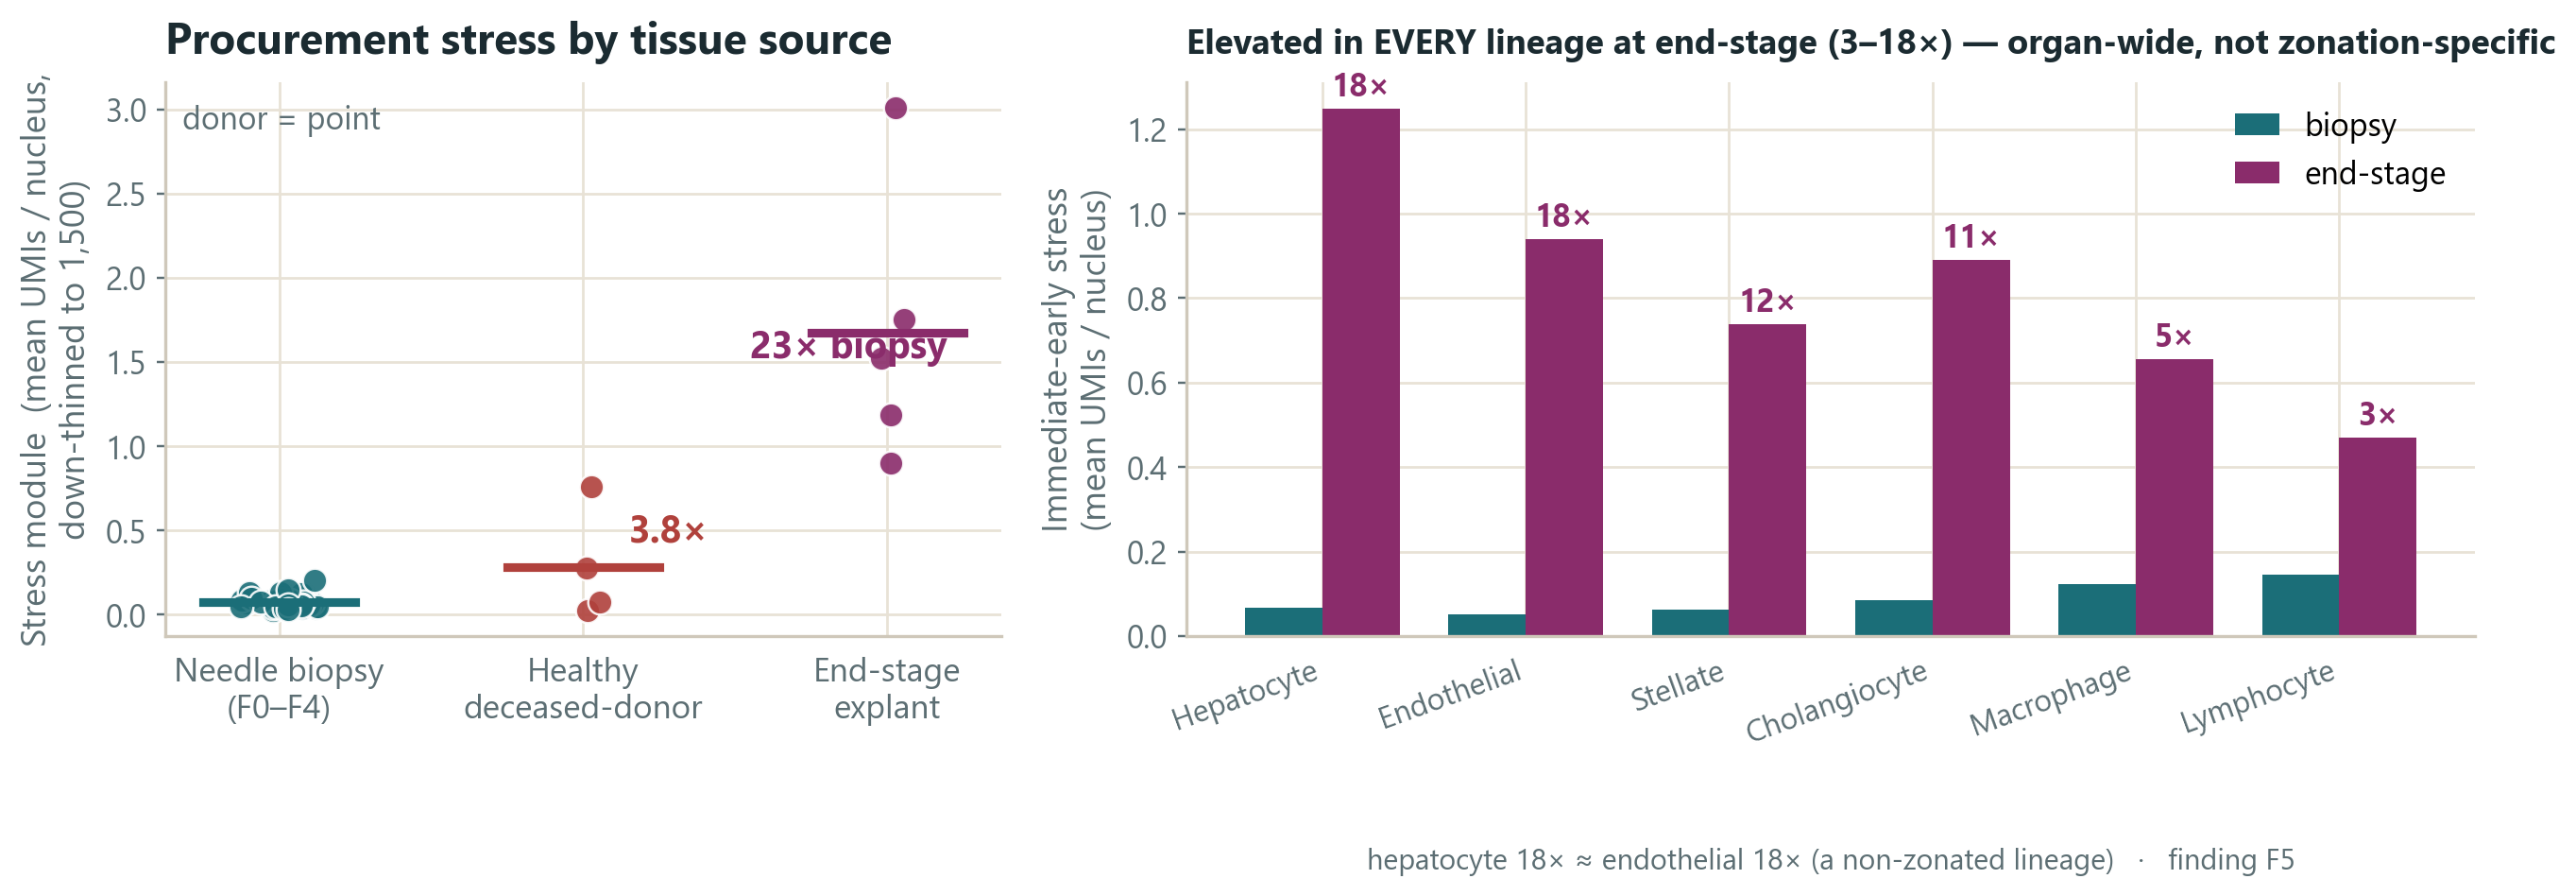
\includegraphics[width=0.85\linewidth]{fig_stress}\caption{Procurement stress by tissue source and across lineages. Depth-matched stress-module (immediate-early $+$ heat-shock) UMIs per nucleus are uniformly low across needle biopsies and rise sharply in the deceased-donor organ-cube endpoints (healthy, end-stage). The explant-vs-biopsy fold is essentially identical in hepatocytes and in endothelial cells, which carry no zonation program --- establishing the signal as organ-wide acute handling, not a hepatocyte disease program.}\label{fig:stress}\end{figure}

\subsection{Matched-biopsy anchor classification preserves zonation}

On the acquisition-matched biopsy axis, every mechanism by which zonation could fail comes up flat. The \textbf{pericentral-anchor fraction} is 36/19/23/22/21\% for F0--F4 --- non-monotone and flat across the disease axis (the F0 value rests on n$=$2 and is descriptive). The \textbf{null} (double-negative) fraction is flat (34/44/36/39/39\%), so identity is not being turned off. The \textbf{PP:PC composition ratio} is 0.62/1.16/1.01/1.10/1.18, flat/non-monotone. Most tellingly, the \textbf{dual co-expression} fraction --- the direct count signature of de-zonation --- collapses from $\sim$7--10\% when a permissive 1-UMI call is used to \textbf{$\sim$0.2--0.6\%} under the ambient-robust $\ge$2-UMI call, with no trend across stage: the apparent co-expression at 1 UMI was ambient soup, not genuine co-detection. For contrast, the same strict $\ge$2-UMI dual fraction in explants is \textbf{$\sim$2.9\% ($\sim$7$\times$) higher}. A broad PC$\leftrightarrow$PP gradient is present at every biopsy stage, including cirrhotic F4; the poles stay dominant.

\begin{figure}[h]\centering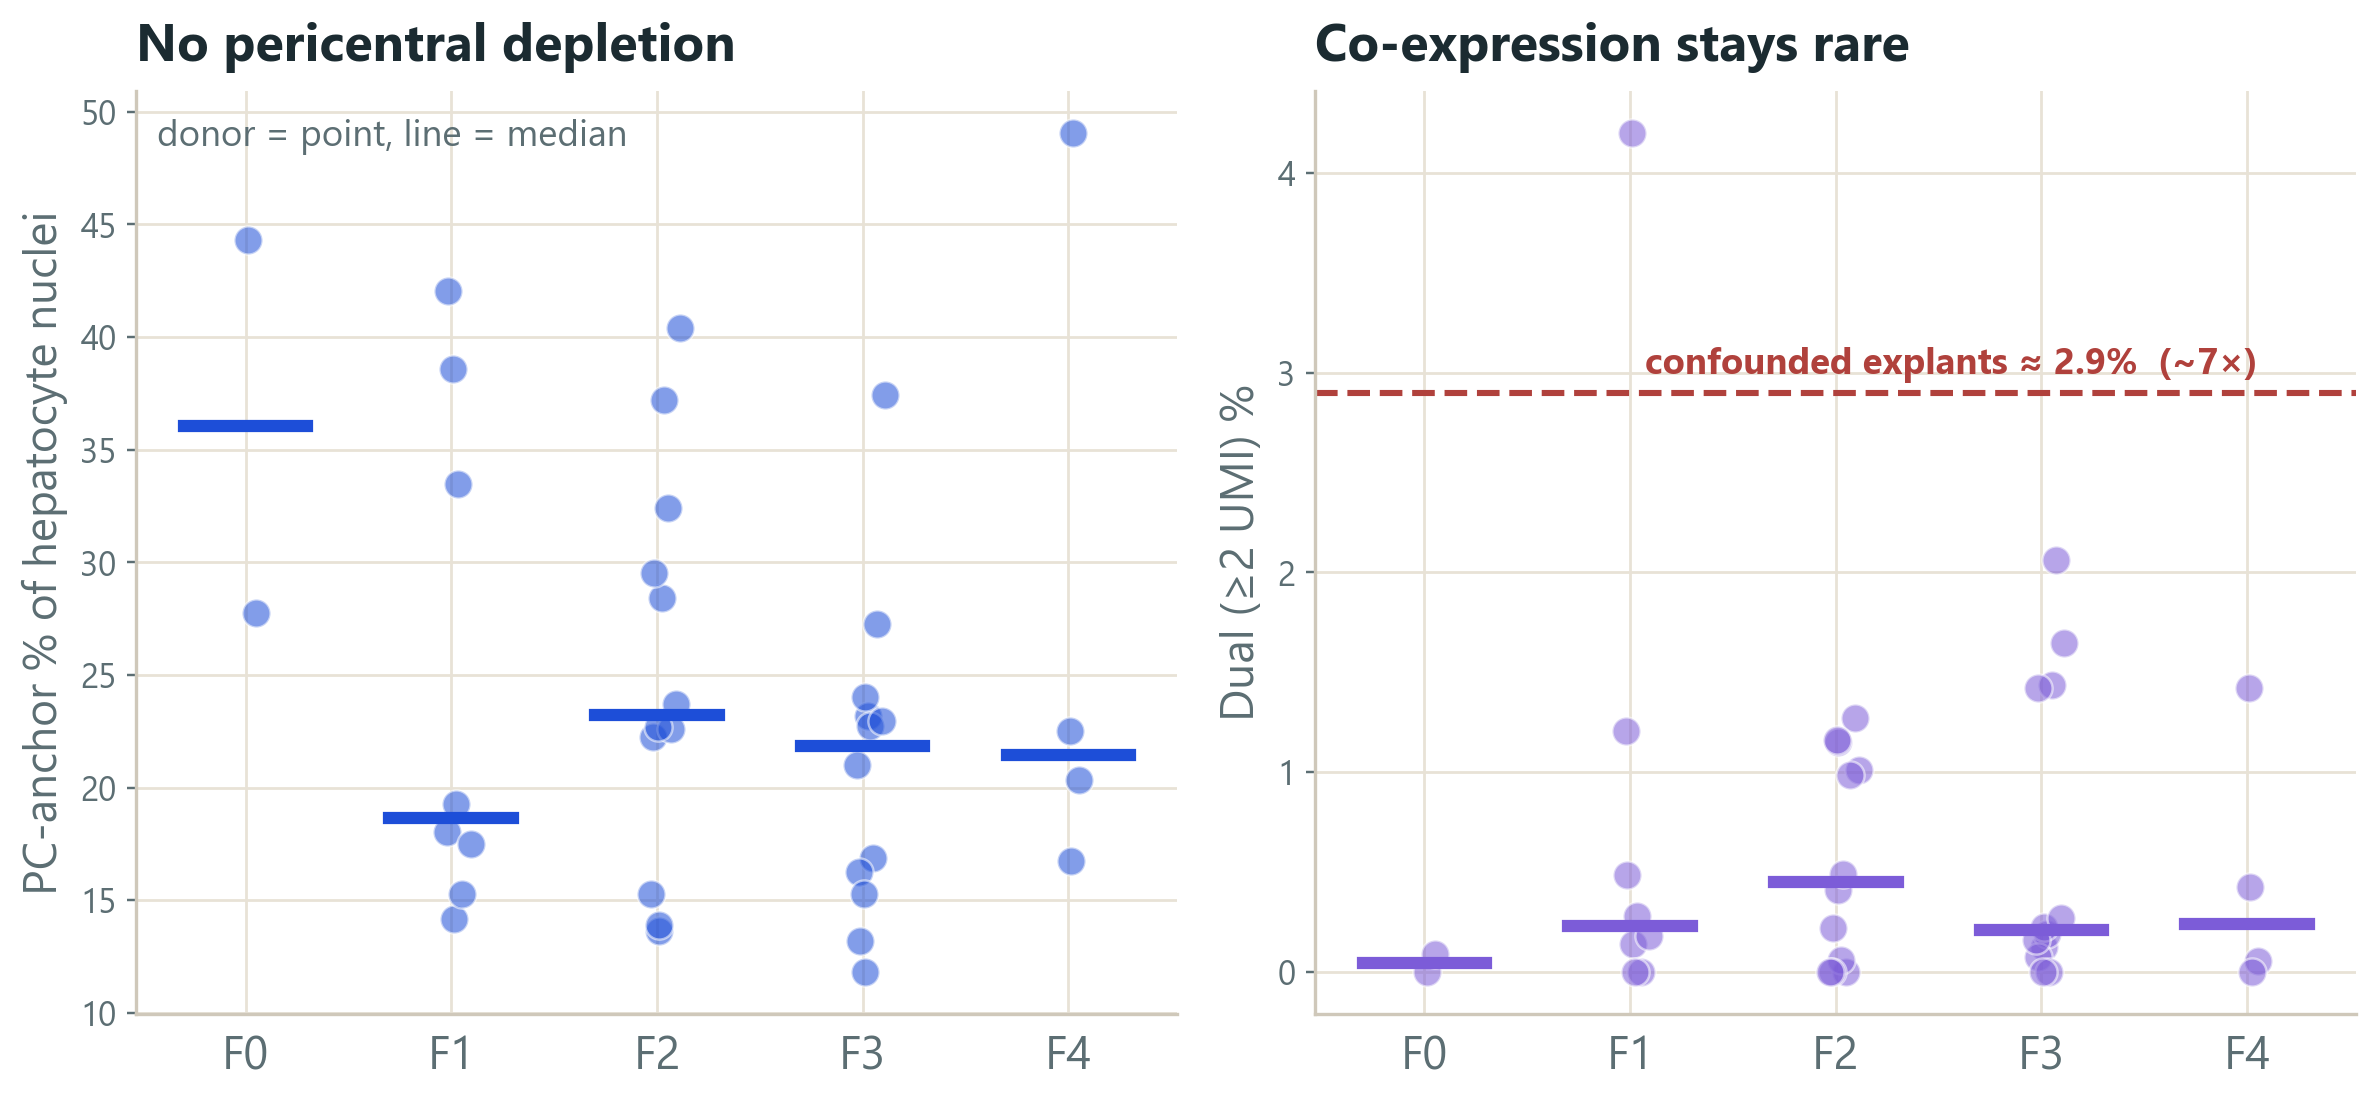
\includegraphics[width=0.85\linewidth]{fig_result2}\caption{Matched-biopsy anchor classification. Pericentral-anchor and strict ($\ge$2-UMI) dual co-expression fractions across needle-biopsy fibrosis stages. The pericentral fraction is flat/non-monotone; the dual fraction is near-zero and collapses from the permissive 1-UMI value, indicating the 1-UMI co-expression was ambient. Full four-panel breakdown (PC / dual / null / PP:PC) in Figure~\ref{fig:anchor2x2}.}\label{fig:result2}\end{figure}

\begin{figure}[h]\centering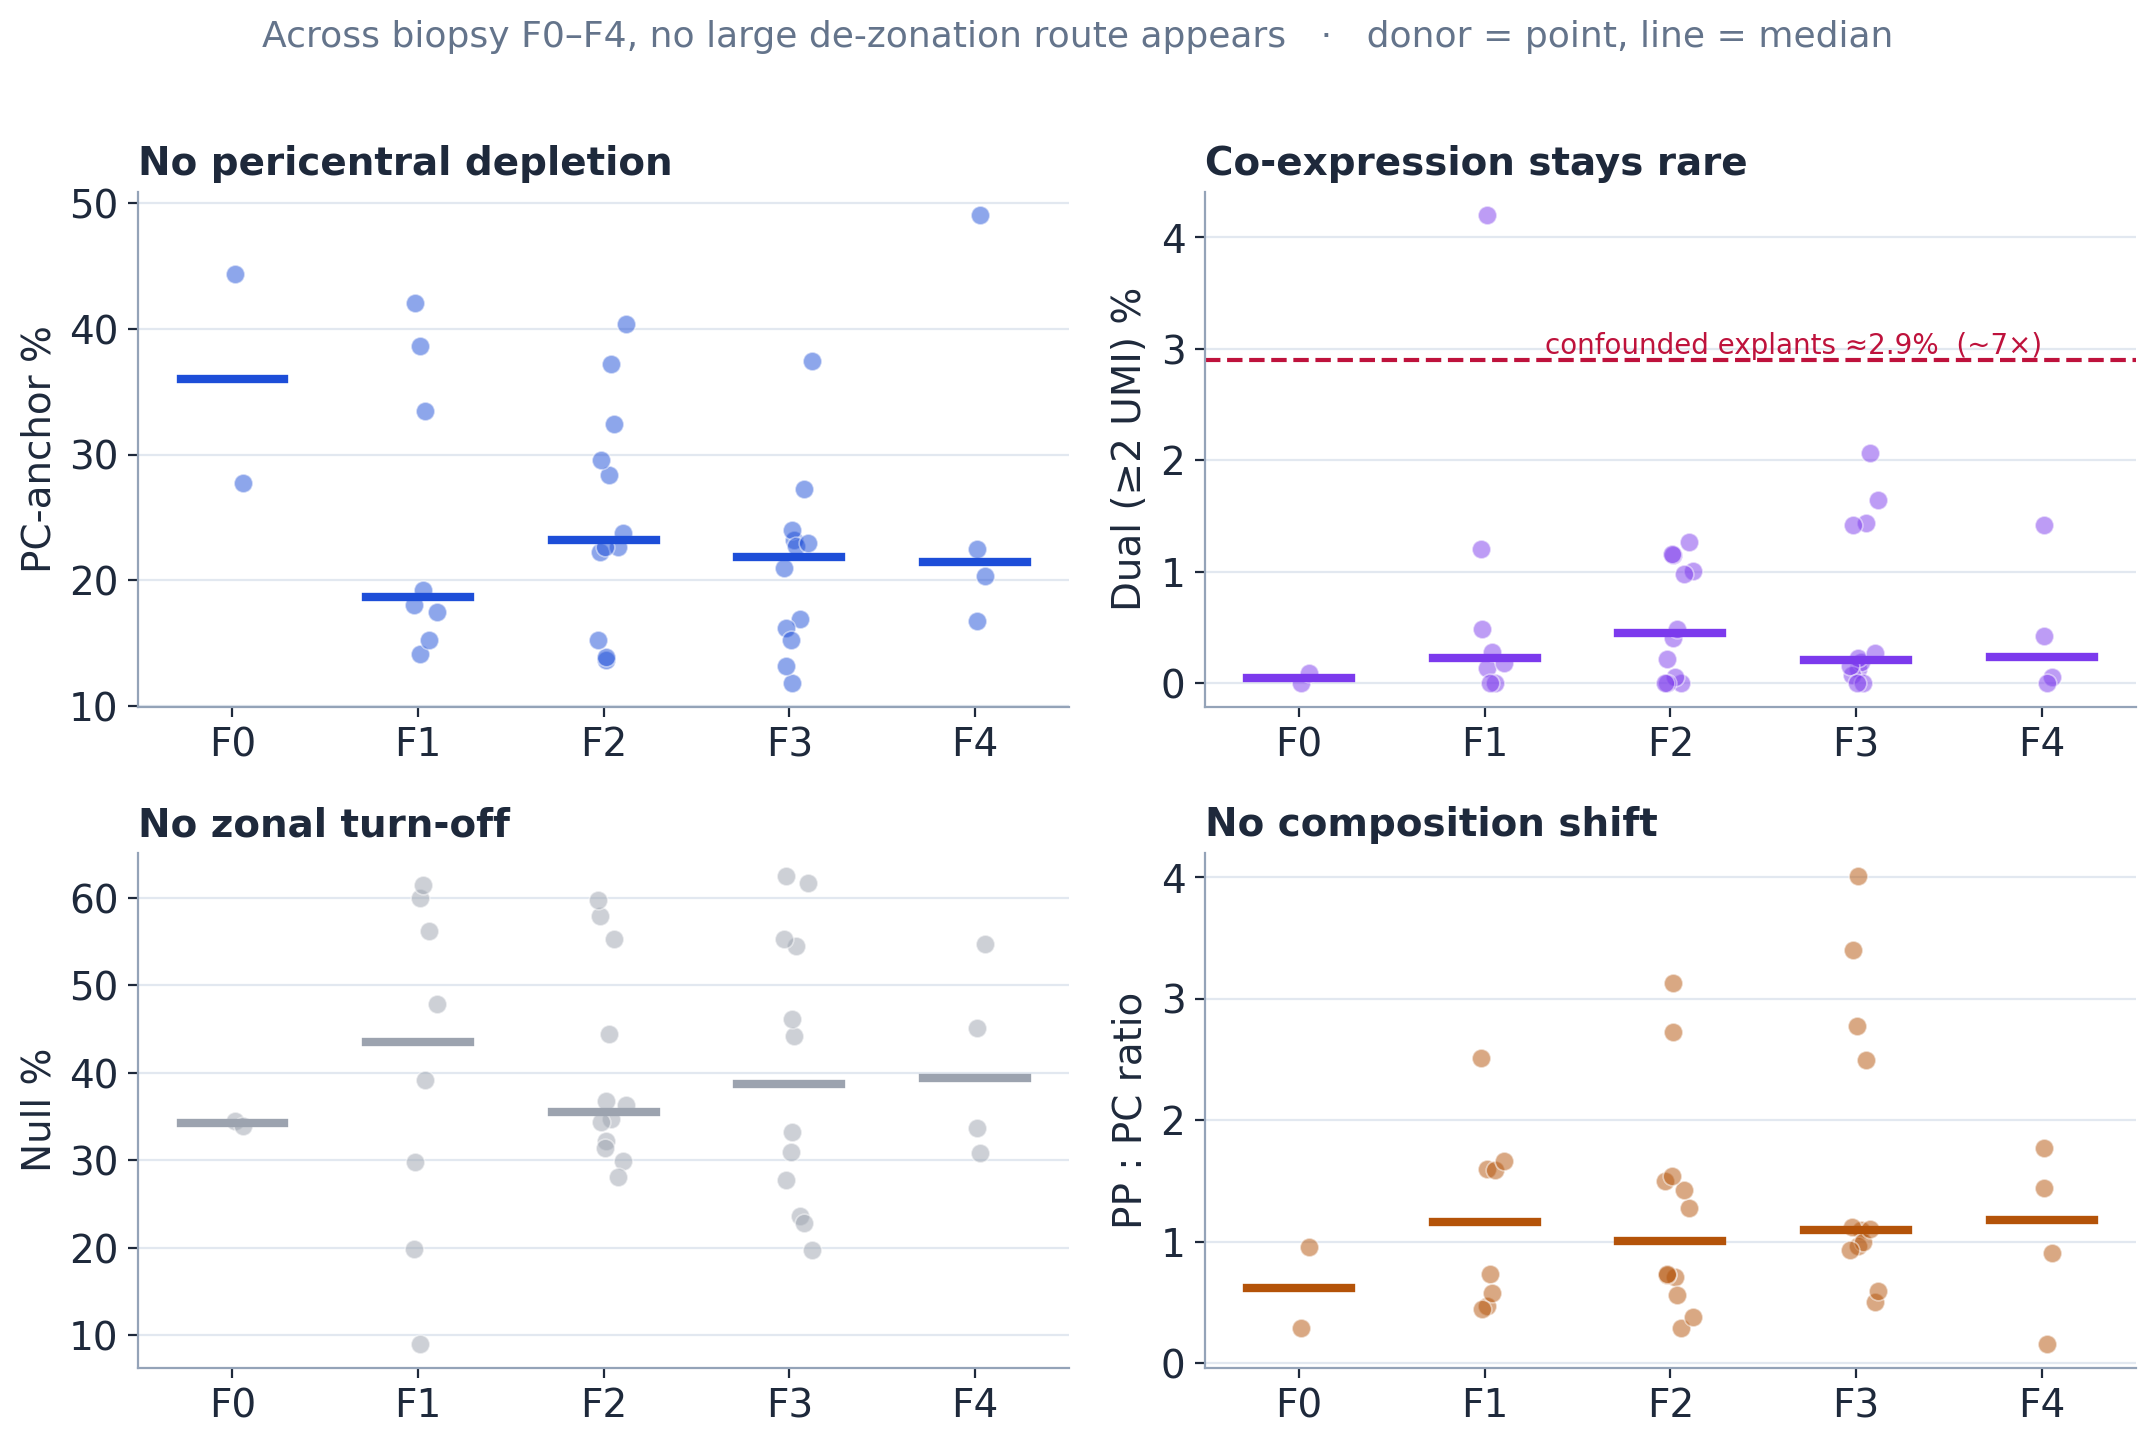
\includegraphics[width=0.85\linewidth]{fig_anchor2x2}\caption{Full anchor 2$\times$2: pericentral-anchor fraction, strict dual co-expression, null (double-negative) fraction, and the periportal:pericentral ratio across biopsy fibrosis stages --- all flat/non-monotone.}\label{fig:anchor2x2}\end{figure}

\subsection{The null is robust and quantitatively bounded}

The preserved-zonation result is not a single fragile contrast. It holds across the entire sensitivity grid (anchor choice, UMI threshold, marker-set ladder from 2 to 1{,}637 genes) with Monte-Carlo SD of 0.006--0.010 on donor-median fractions. To bound it affirmatively, a TOST equivalence test on the donor-level pericentral-anchor fraction gives an F4-vs-F1 difference of \textbf{$+$0.024 ($+$2.4 percentage points), 90\% CI $-$0.147 to $+$0.194}; the better-powered interior F1-vs-F3 tightens to roughly $\pm$0.12. In words: the matched axis \textbf{excludes a large coordinated re-zonation on the order of 20 percentage points}, but \textbf{does not exclude a subtle drift of $\le$$\sim$10 points} (the donor-level SD at n$=$4 is too large to rule that out). This is a bounded null --- large/dramatic collapse excluded; subtle change not excluded --- and the bound applies to donor-level transcriptional \emph{structure}, not to lobule-scale spatial architecture, which snRNA cannot see.

\begin{figure}[h]\centering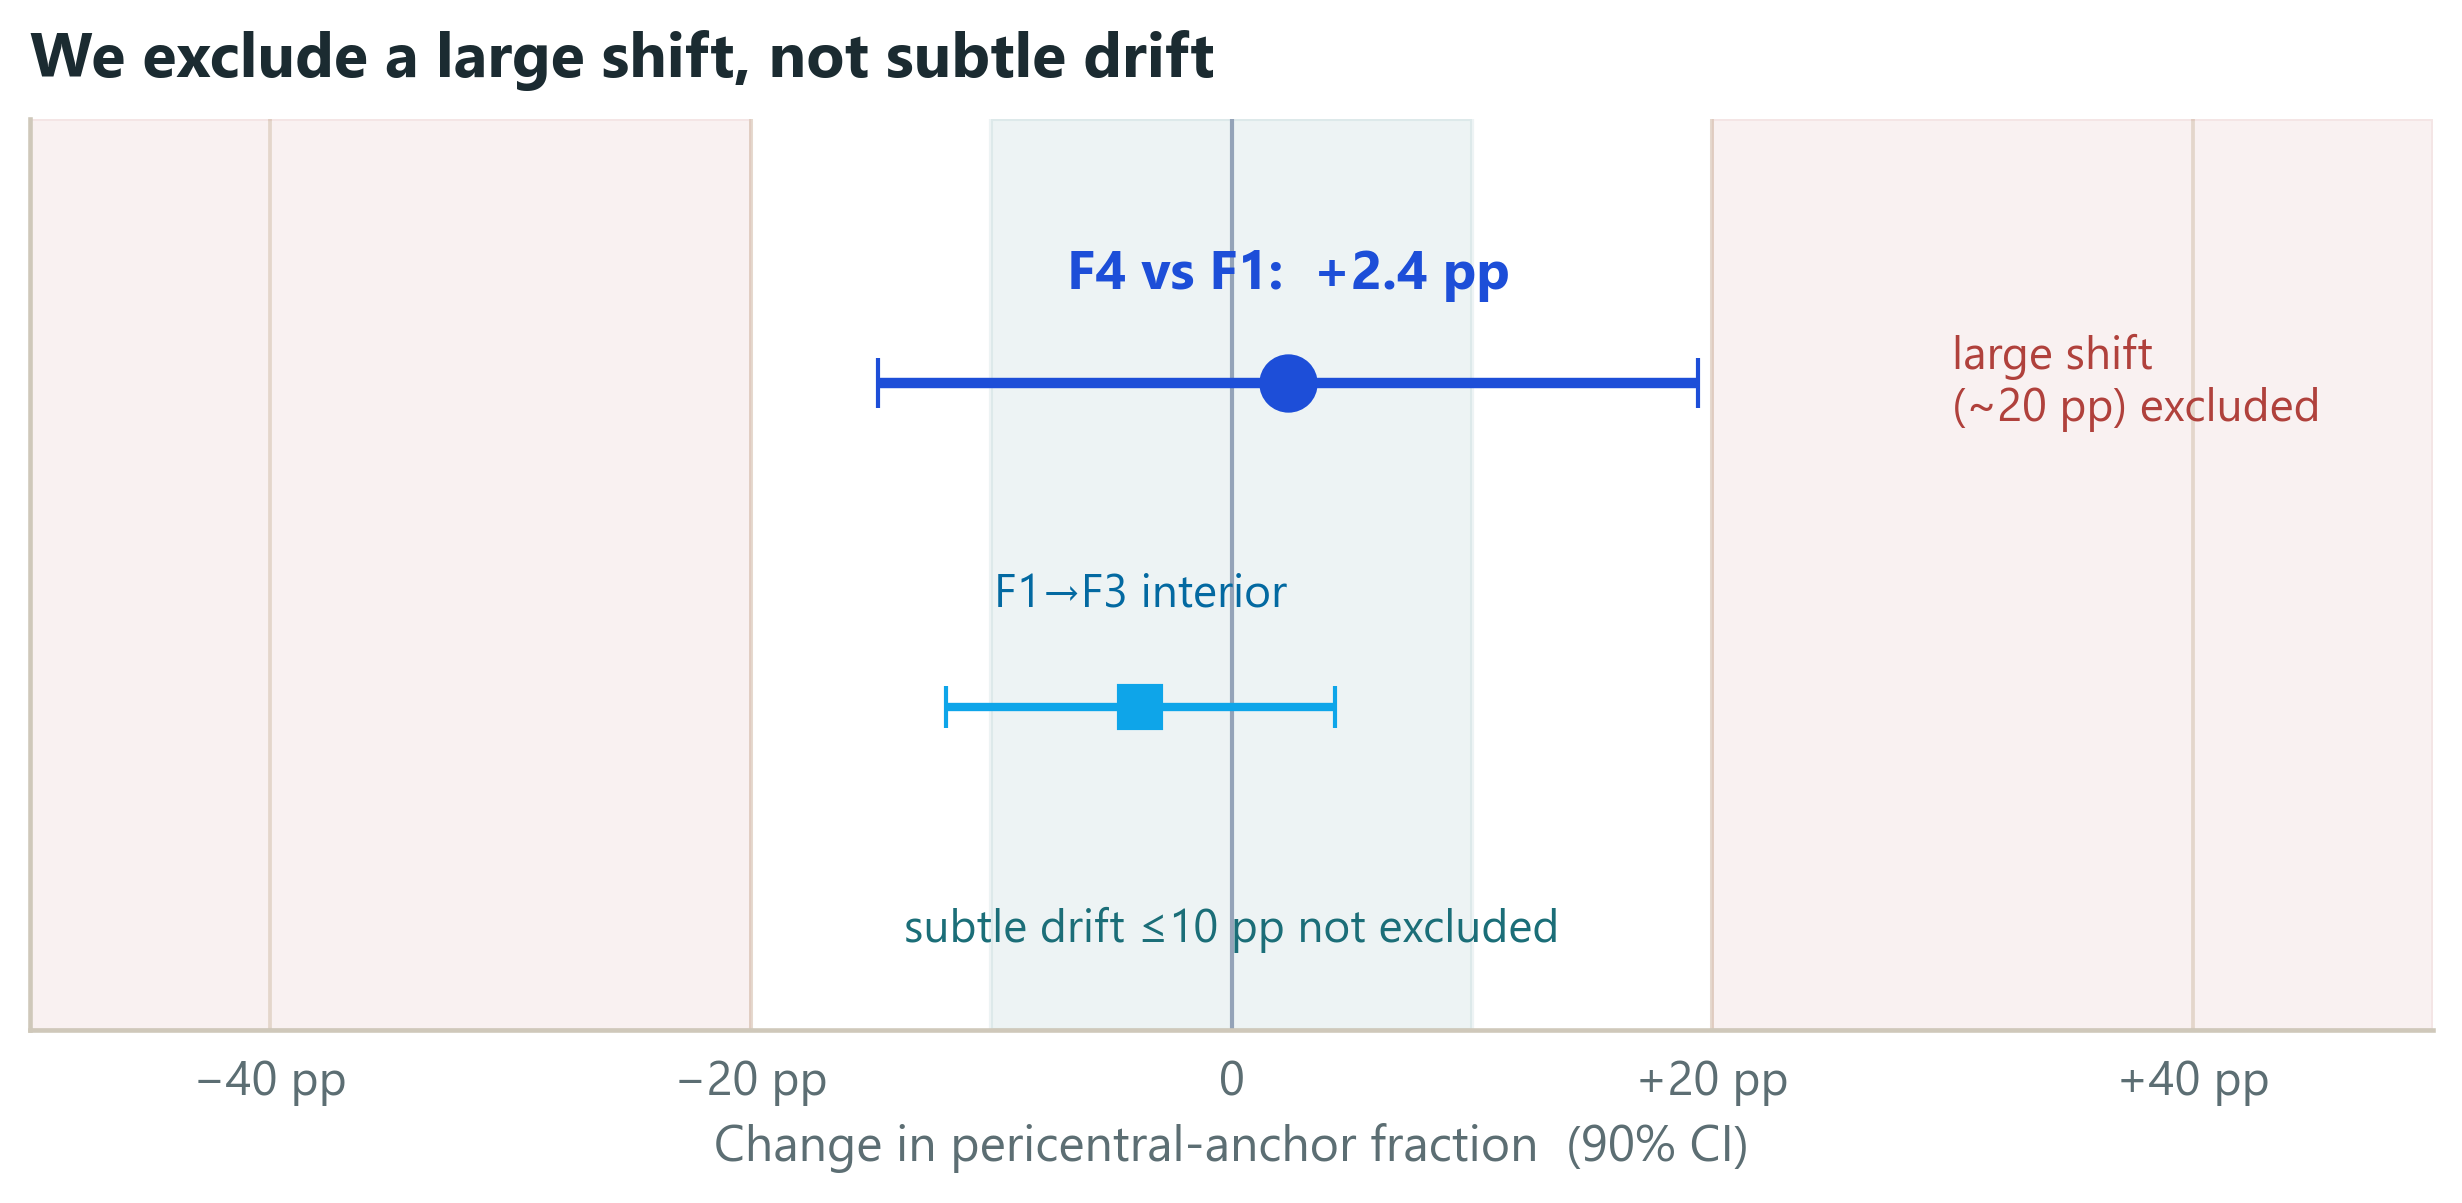
\includegraphics[width=0.85\linewidth]{fig_tost}\caption{Equivalence bound. TOST on the donor-level pericentral-anchor fraction across biopsy F1$\to$F4: the 90\% CI excludes a $\sim$20-point shift but not a $\le$10-point drift --- a quantified bound on ``preserved,'' honest about the limited power at n$=$4.}\label{fig:tost}\end{figure}

\subsection{End-stage explants are heterogeneous, not one program}

Setting the explants aside as confounded does not mean they are uninformative about \emph{why} pooling fakes a collapse. The five explants go in opposite directions rather than sharing one end-stage phenotype: \textbf{CL104} retains its pericentral pole (PC-anchor 49.7\%, PP:PC 0.13); \textbf{CL16} nearly collapses to periportal (PC 3.2\%, PP:PC 20.3); \textbf{CL18} floods into co-expression (dual 22.4\%); CL103 and CL17 are periportal-leaning. Across the five, the pericentral-anchor fraction spans 3--50\% and PP:PC spans 0.13--20. Pooling five discordant organs into one marker correlation manufactures a single uniform ``collapse'' that none of them individually shows --- the signature of heterogeneous, separately-handled organ procurement.

\begin{figure}[h]\centering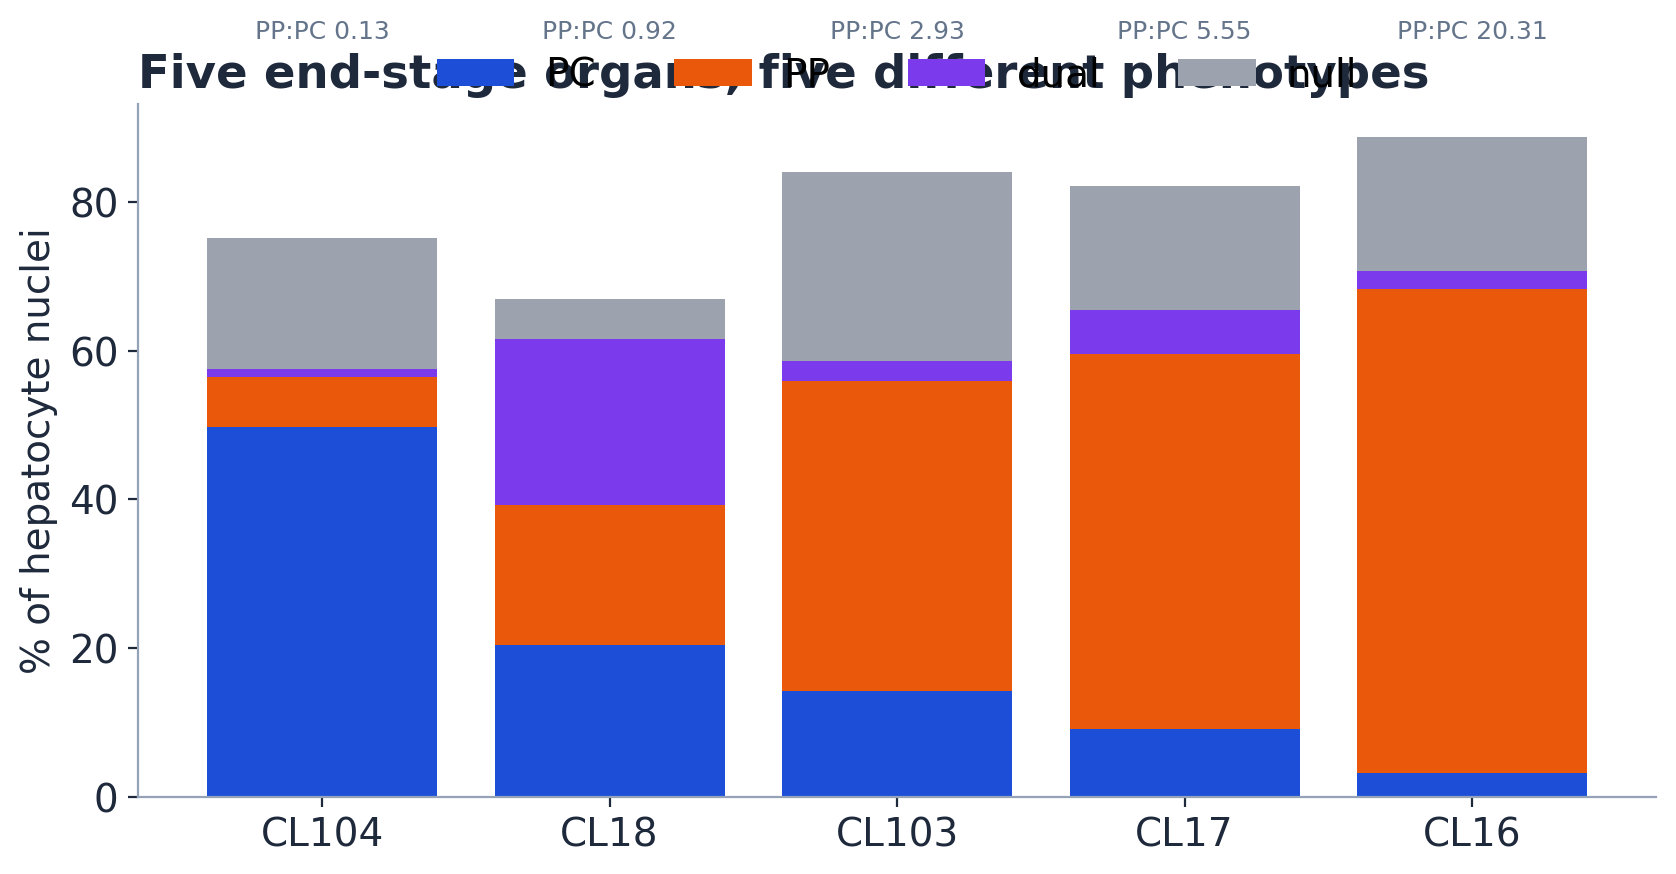
\includegraphics[width=0.85\linewidth]{fig_explant}\caption{End-stage explant heterogeneity. Per-explant anchor profiles: the five organs span retained pericentral identity (CL104) to near-total periportal collapse (CL16) to a co-expression flood (CL18). A pooled correlation collapses these into one number.}\label{fig:explant}\end{figure}

\subsection{Genome-wide DGE finds a biliary burden, not zonation loss}

A genome-wide donor-level pseudobulk DGE scan plays two roles. As an \textbf{independent count-based check} on the zonation result, the zonation genes are flat at the expression level --- GLUL FDR \textbf{0.80}, CYP3A4 0.85, ASS1 0.96, with all detox/periportal markers FDR $>$ 0.79 --- agreeing with the anchor classification (this is a corroborating sanity check, \emph{not} the primary proof). As a \textbf{discovery scan}, of the 21{,}022 tested genes only \textbf{64 reach FDR$<$0.05 at F4-vs-F1} (omnibus across stages: 91), and they form a coherent \textbf{biliary/ductular marker burden}: EPCAM (logFC $+$2.3, FDR 0.002), GRHL2 ($+$3.1, FDR 0.0004), SPINT2 ($+$2.7, FDR 0.003), SOX4 ($+$2.5, FDR 0.047), SOX9 ($+$2.4, FDR 0.044), B3GNT3 ($+$2.9, FDR 0.001), plus CXCL10 ($+$5.4, FDR 0.001). The honest claim is bounded: \textbf{no large single-gene hepatocyte program changes across the matched axis other than this biliary burden} --- but a gene-level scan can miss a weak \emph{coordinated} program (tens-to-hundreds of genes each shifting modestly without any one crossing FDR), so a gene-set test is still owed (see Sec.\ 4.4, 4.6). A within-class confirmatory DGE (Plan B) found the same biliary set appearing class-agnostically across PC/PP/null/dual nuclei, with zonation genes flat inside every class.

\begin{figure}[h]\centering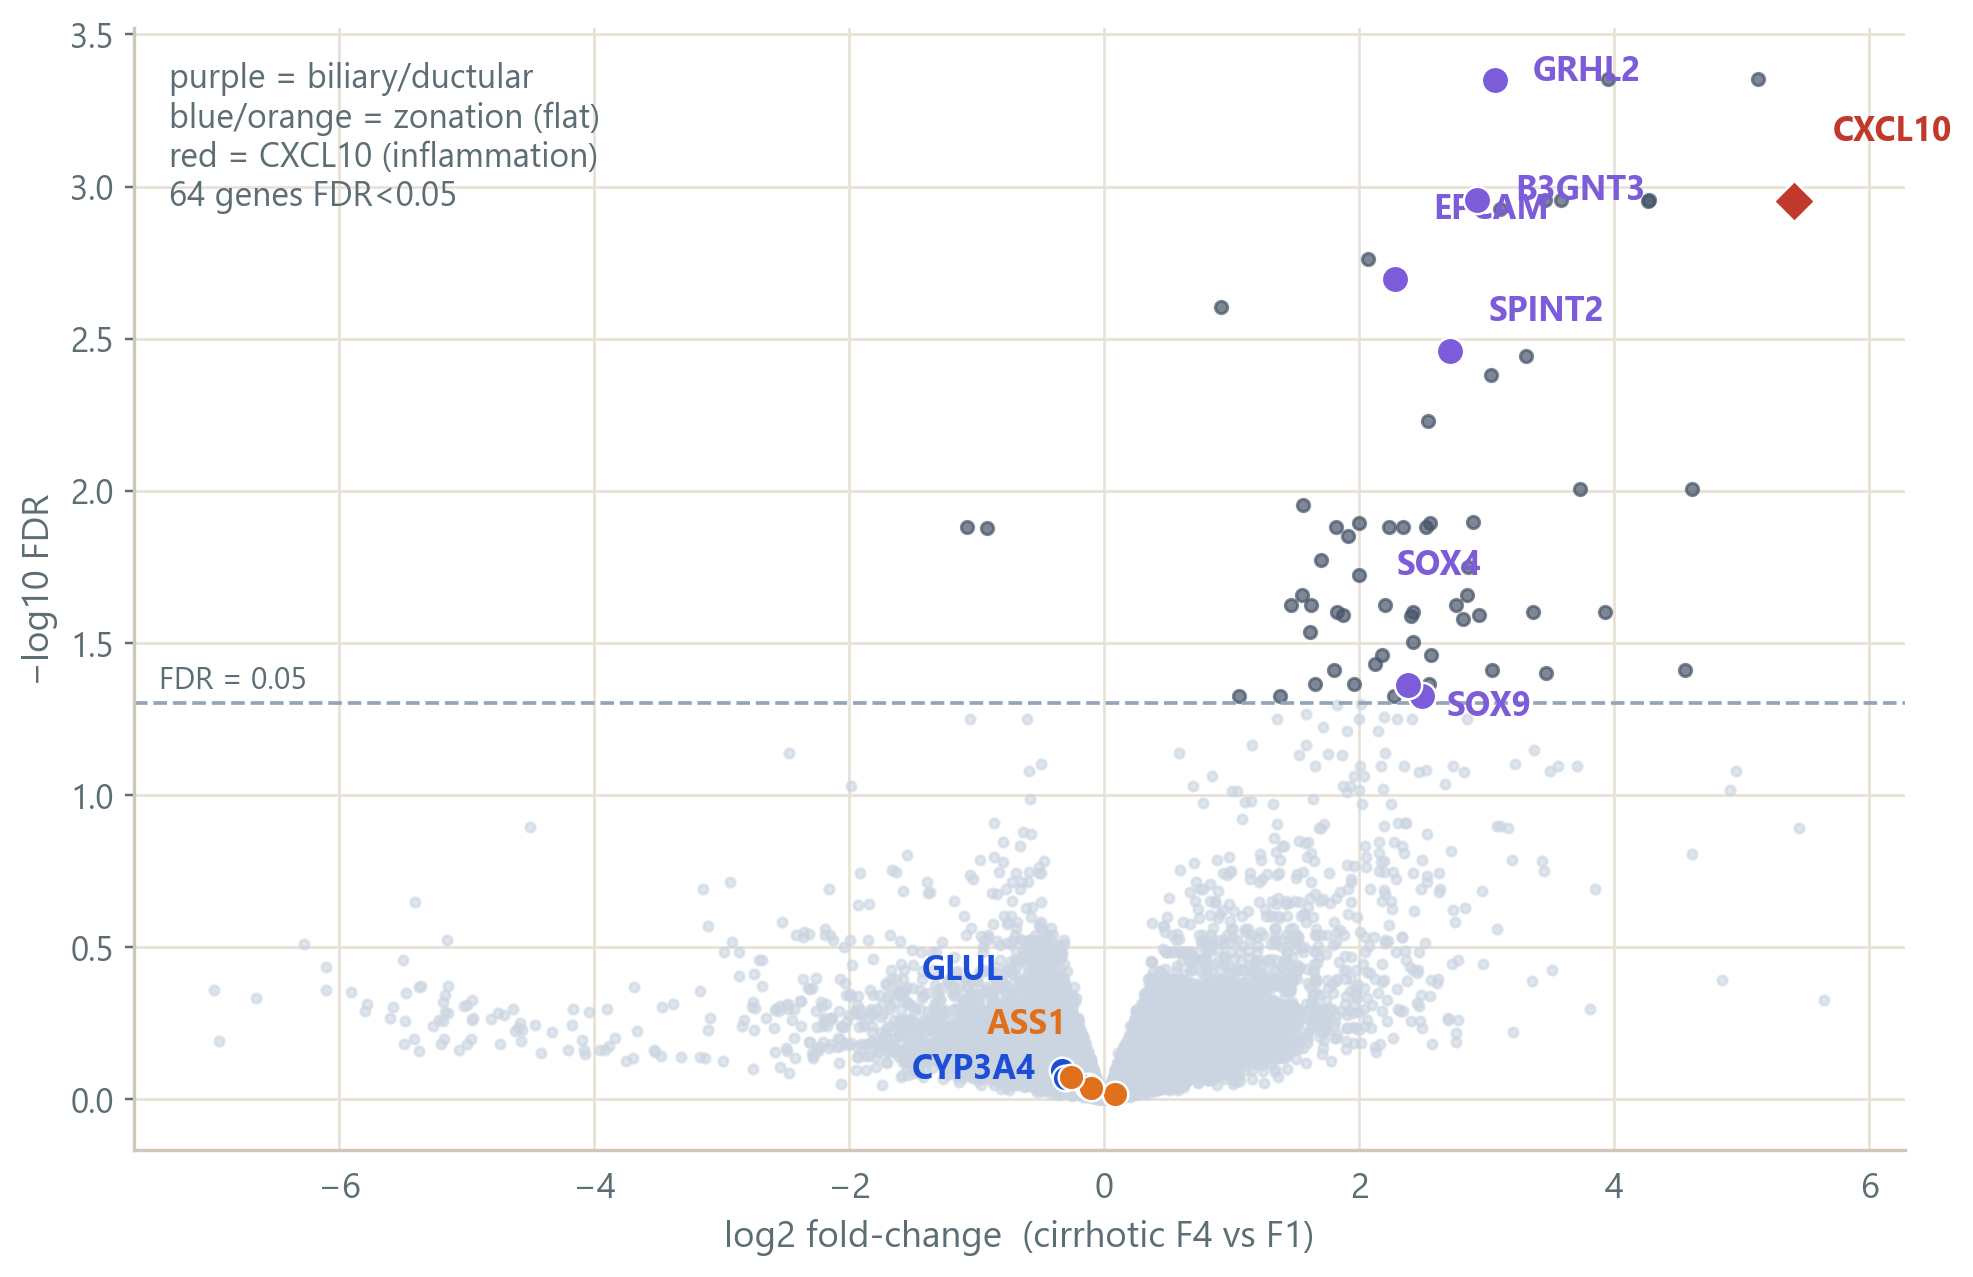
\includegraphics[width=0.85\linewidth]{fig_volcano}\caption{Genome-wide pseudobulk DGE (F4-vs-F1) volcano. Zonation genes sit at the origin (flat; GLUL FDR 0.80). The significant hits are a biliary/ductular marker set (EPCAM, GRHL2, SPINT2, SOX4, SOX9, B3GNT3) plus CXCL10.}\label{fig:volcano}\end{figure}

\subsection{The biliary burden is most consistent with a compositional source --- a lead, not a verdict}

Several lines of evidence point to the biliary burden being \textbf{compositional} rather than hepatocyte-intrinsic transdifferentiation, but none closes the question. (i) Every headline biliary gene is \textbf{5--78$\times$ more abundant in cholangiocytes than in hepatocytes} --- the profile of ambient soup. (ii) The cholangiocyte fraction itself rises to \textbf{$\sim$8\% at F4} (the expected ductular reaction), so a per-cell-fraction ``rise'' in hepatocyte-labeled pseudobulk is exactly what compositional spillover predicts. (iii) Only \textbf{$\sim$0.4\%} of hepatocyte nuclei robustly co-express $\ge$2 biliary markers --- too few to drive a widespread program. (iv) \textbf{decontX} cuts the hits from 64 to 34 and drops the canonical plasticity factors \textbf{SOX4 (FDR 0.131) and SOX9 (FDR 0.118)} below significance, while \textbf{EPCAM, B3GNT3, SPINT2 and CXCL10 survive} --- consistent with a mixed source, but decontX uses the paper's own labels and can over- as well as under-correct, so it \emph{demotes, it does not disprove}, these genes. A crude doublet probe (hepatocyte-cholangiocyte co-capture suspects, KRT19/KRT7 $\ge$2 UMI) rises $\sim$17$\times$ with fibrosis and carries the inflated-total-count signature of genuine co-capture, yet all such nuclei sit \emph{below} the paper's only doublet filter (0 of 42{,}579 biopsy hepatocyte nuclei exceed the $>$50{,}000-count cutoff) --- an illustrative lead that cannot separate a doublet from a rare transdifferentiating cell. \textbf{CXCL10 is carved out separately}: its hepatocyte expression does not track the cholangiocyte fraction (correlation $-$0.09), so it is a \emph{candidate real inflammatory signal}, not ambient. Net reading: the biliary burden is \textbf{most consistent with cholangiocyte ambient RNA plus a small fibrosis-rising co-capture/biphenotypic contribution that Paper 1's filter could not have removed} --- neither hepatocyte-intrinsic --- but the source attribution is an open lead, repeatedly flagged as such, not a closed result.

\begin{figure}[h]\centering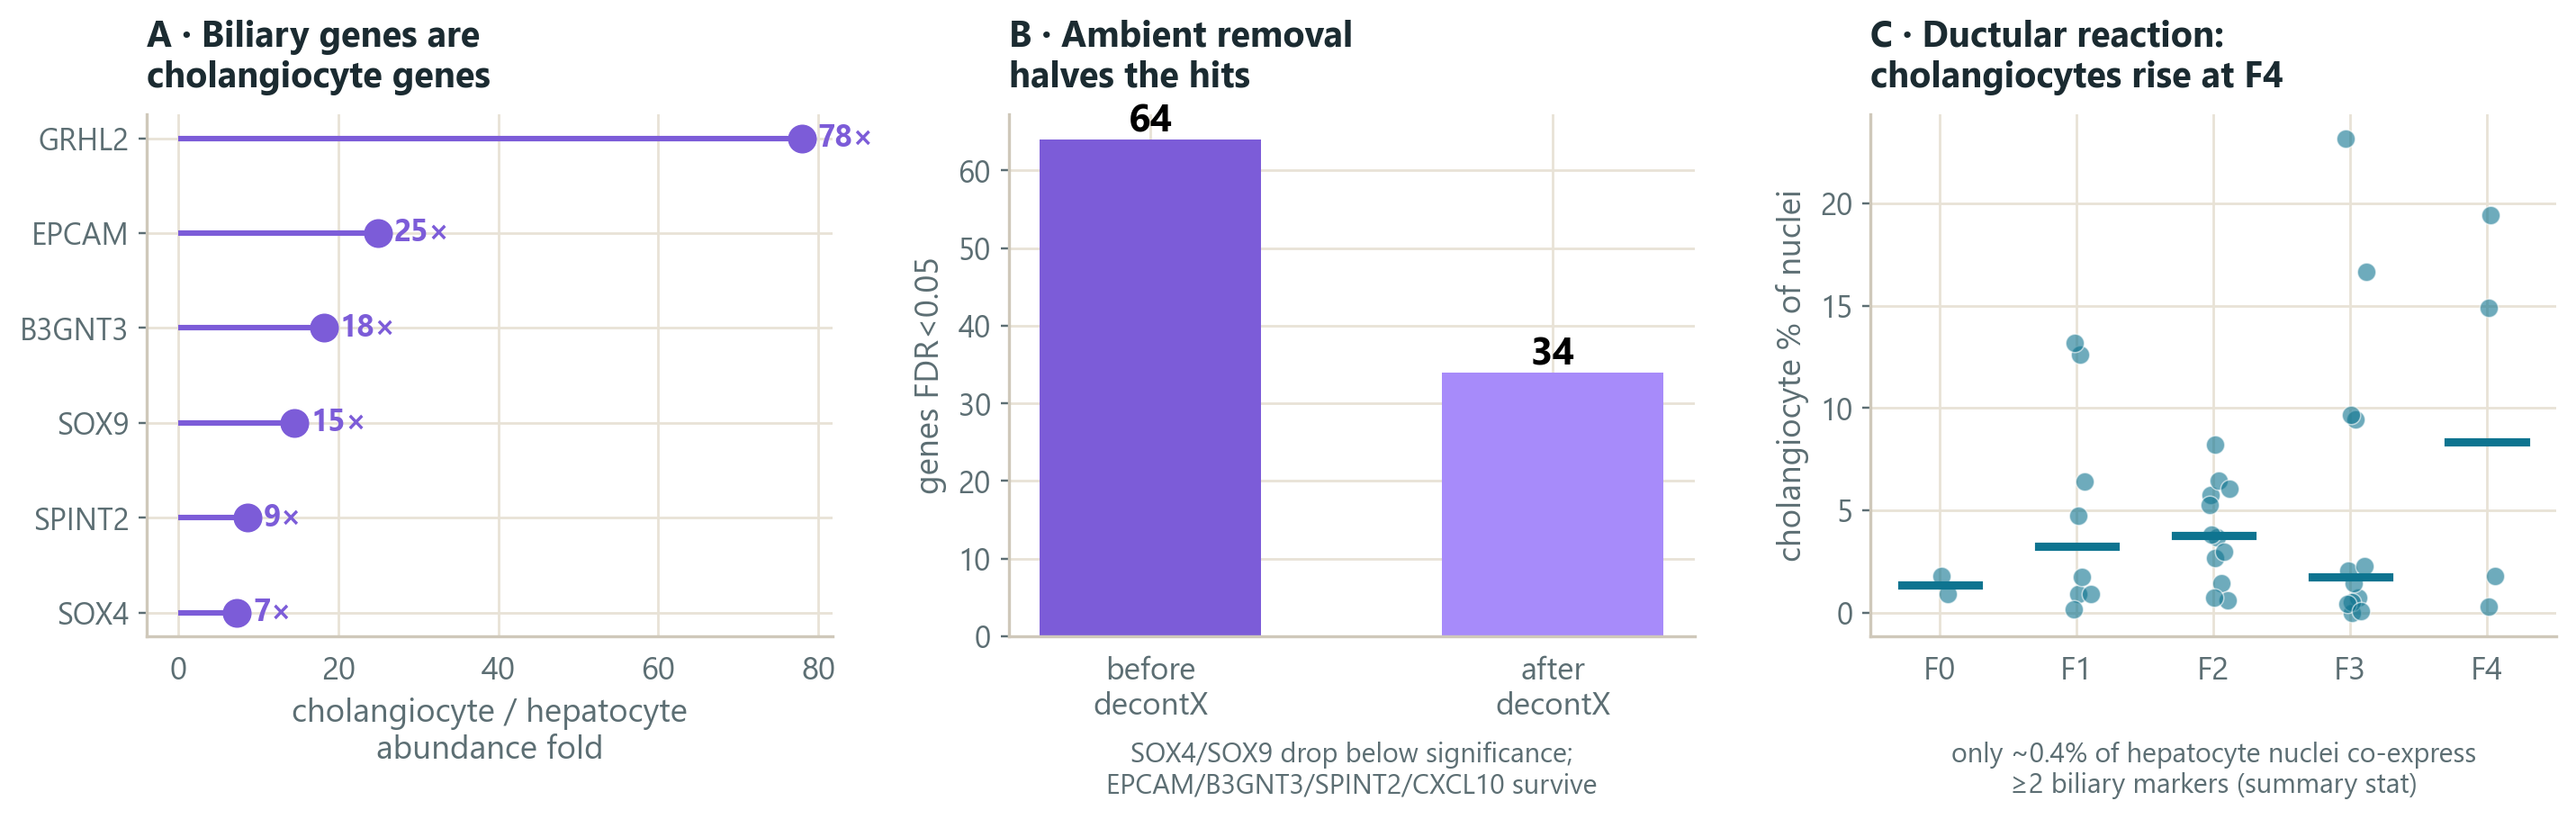
\includegraphics[width=0.85\linewidth]{fig_compositional}\caption{Source attribution of the biliary burden (3-panel). Left: headline biliary genes are 5--78$\times$ cholangiocyte-dominant across lineages. Middle: cholangiocyte fraction rises into F4 (ductular reaction). Right: decontX reduces hits 64$\to$34, dropping SOX4/SOX9; EPCAM/B3GNT3/SPINT2/CXCL10 survive. Most consistent with a compositional source; not a closed verdict.}\label{fig:compositional}\end{figure}

\begin{figure}[h]\centering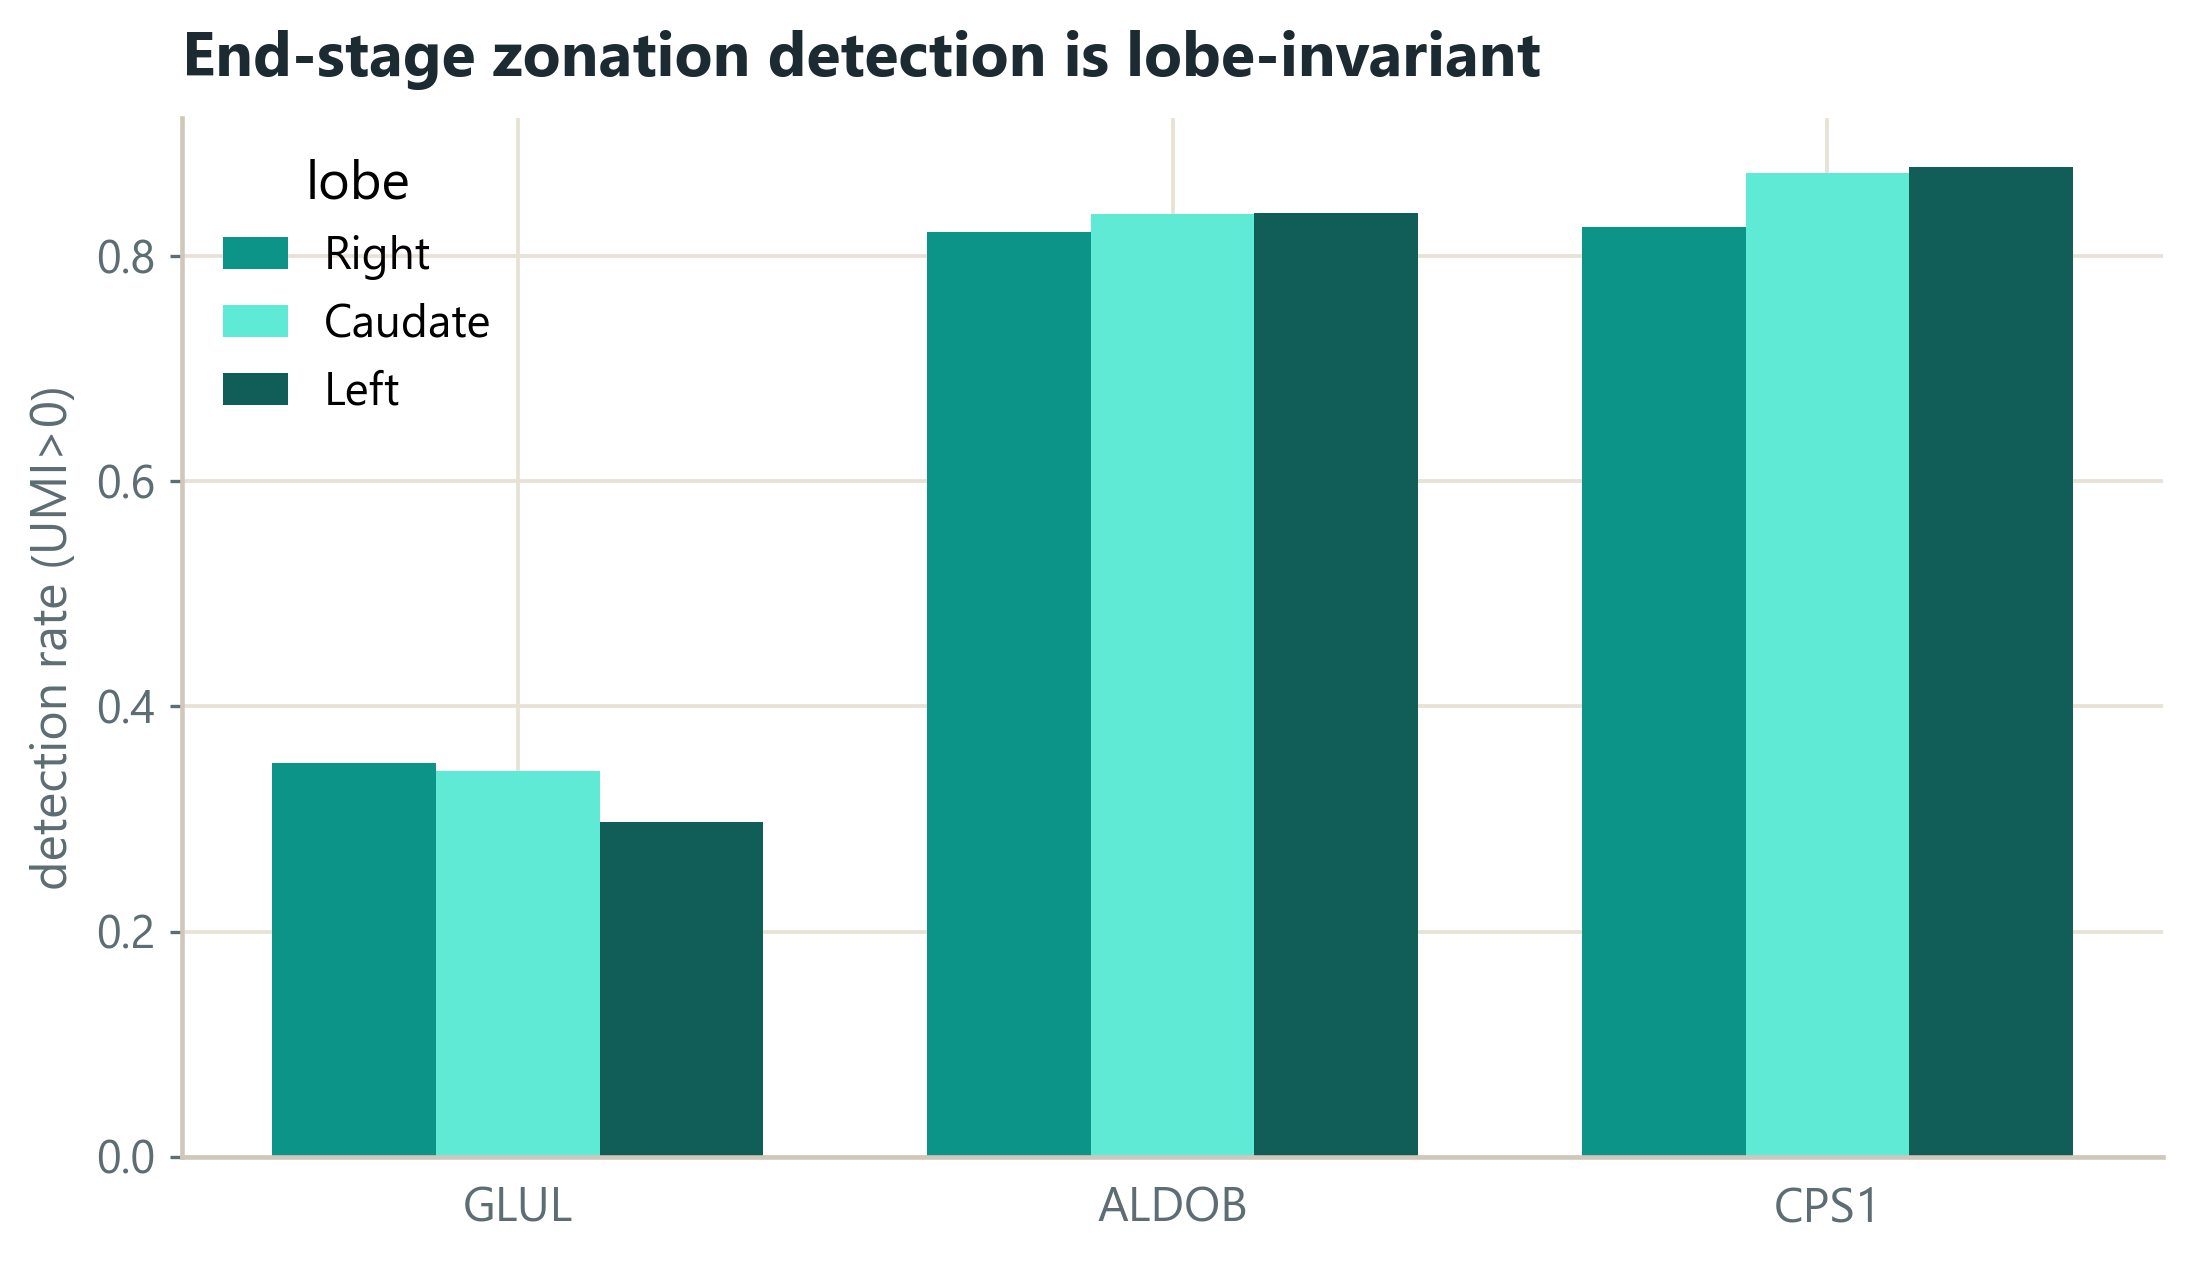
\includegraphics[width=0.85\linewidth]{fig_lobe}\caption{Lobe invariance (supporting). Within explants, the zonation-marker detection pattern is invariant across right/caudate/left lobes (e.g.\ GLUL 0.350/0.343/0.297), so multi-lobe sampling does not manufacture the de-zonation signal --- clearing one sub-confound.}\label{fig:lobe}\end{figure}

\textbf{Two conceptual figures} belong with this report but are not fabricated here. A \textbf{study-design / confound schematic} would show the disease axis (F0--F4 needle biopsies, right lobe) beside the endpoints (healthy and end-stage deceased-donor organ cubes, multi-lobe), with the stage-vs-acquisition collinearity stated explicitly: because every milder sample is a biopsy and every end-stage sample is an explant, disease stage and acquisition method are perfectly collinear and not separable in the pooled comparison \emph{(schematic; see presentation slides 3 and 5)}. An \textbf{anchor-method pipeline schematic} would show raw counts $\to$ binomial down-thinning to 1{,}500 UMIs $\to$ $\ge$2-UMI strict anchor calls $\to$ PC/PP/dual/null per nucleus $\to$ donor-level fractions $\to$ sensitivity grid \emph{(schematic; see presentation slides 5 and 8)}.

\FloatBarrier
\section{Discussion}

\subsection{Summary}

Three results, at three confidence levels. \textbf{Main result:} across acquisition-matched needle-biopsy MASLD (F1$\to$cirrhotic F4), hepatocyte transcriptional zonation is preserved against any large change --- the anchor classification is flat across the full sensitivity grid, and an equivalence test excludes a $\sim$20-point coordinated shift (interior $\sim$12 points), while not excluding a $\le$10-point drift. The dramatic de-zonation in the pooled analysis is largely a tissue-acquisition confound: the signal lives in deceased-donor organ tissue carrying organ-wide procurement stress, and within the explants it is heterogeneous rather than one program. \textbf{Secondary result:} the one genome-wide change across the matched axis is a biliary/ductular marker burden (64 hits) inside hepatocyte-labeled pseudobulk; zonation genes are flat (GLUL FDR 0.80). \textbf{Interpretive lead:} that burden is most consistent with cholangiocyte ambient RNA plus rare mixed/doublet nuclei, with CXCL10 a separate candidate inflammatory signal --- a promising but unclosed source attribution. \textbf{Limitation:} the gene-level scan does not exclude a weak coordinated program; gene-set testing is owed.

\subsection{Meaning for liver biology}

The matched-biopsy null says that, at the level snRNA can measure --- per-cell transcriptional \emph{balance} between the two zonal programs --- hepatocytes in biopsy MASLD, up to and including cirrhotic-F4 needle tissue, still maintain a broad pericentral$\leftrightarrow$periportal gradient with distinct, dominant poles. This does not contradict the existence of an end-stage phenotype; it relocates it. The strong transcriptional signal is an end-stage / explant phenomenon, exactly as the paper's own figure scoping (``\ldots in end-stage MASLD'') suggests, and it co-occurs with whole-organ acute stress. The biliary burden, read compositionally, is consistent with the ductular reaction (more cholangiocytes, more soup) rather than wholesale hepatocyte reprogramming --- but the unresolved co-capture/biphenotypic fraction leaves room for a small intrinsic contribution that this cohort cannot quantify.

\subsection{Relation to the original paper}

This is a correction of one evidence leg, not an overturning. We re-examine only the \textbf{single-nucleus transcriptional} de-zonation statistic --- a relative marker correlation pooled across a sampling discontinuity --- and find that, on acquisition-matched biopsy tissue and raw counts, it does not support \emph{progressive, disease-driven} de-zonation. We explicitly do \textbf{not} touch the paper's immunofluorescence (GLUL/ASS1 co-localization), its whole-organ FLASH 3D imaging of end-stage architecture, or its organoid / PI3K-AKT-mTOR plasticity evidence; those measure different molecules and timescales than the acute RNA signal we analyse, and cirrhosis genuinely remodels the lobule. We also agree with the paper that the strong signal is an end-stage phenomenon --- which is precisely the tissue we set aside as confounded. The disagreement is narrow: the \emph{transcriptional} de-zonation does not appear in matched biopsy tissue, and the modest biopsy-stage biliary rise is most consistent with a compositional source rather than hepatocyte-intrinsic transdifferentiation.

\subsection{Limitations}

The matched axis is small at its extremes (F0 n$=$2, F4 biopsy n$=$4), so the equivalence bound rules out only large shifts --- a $\le$10-point drift is not excluded. snRNA measures per-cell transcriptional balance, \textbf{not lobule geometry}; needle cores miss septa and perivenular zones, so we claim transcriptional, not spatial/architectural, preservation. Sequencing batch is not randomized (V(run, source)$=$0.84); within the biopsy axis the biliary hits survive a run covariate and a single-run test, so they are not a batch artifact, but the design is not clean. decontX is a consistency check carrying mild circularity (it uses the paper's labels), and the doublet probe is an exploratory lead (n$=$16 suspects) that cannot separate a doublet from a rare transdifferentiating cell. Most importantly, the genome-wide claim is \textbf{gene-level}: a weak coordinated program could hide below per-gene FDR, so ``no other hepatocyte program'' must travel with that caveat until gene-set testing is done. This is a single cohort with no independent biopsy series and no protein/spatial validation of our own.

\subsection{Challenges and lessons learned}

The project's own progression record (archived deck and primer) documents a real methodological turn. The original instrument was a \textbf{relative, z-scored zonation ``ruler''} built from a healthy spatial atlas and applied via marker correlation --- and it produced the apparent collapse. Two problems retired it. First, it was \textbf{source-confounded}: pooled across the needle-biopsy$\leftrightarrow$organ-cube discontinuity, it manufactured a between-group ``collapse'' that dissolved within groups --- a textbook Simpson's-paradox reversal (each healthy donor individually anti-correlated, yet pooling the four flipped the sign). Second, it was \textbf{intrinsically depth-sensitive and mechanism-blind}: turn-off, co-expression and pure noise all shrink a z-scored spread identically, so the ruler could not say \emph{how} zonation was changing. The fixes followed directly: move to \textbf{raw molecule counts} (the shipped matrix is an SCT output, unusable for co-detection and ambient sensitivity); equalize sequencing depth by \textbf{binomial down-thinning} so detection differences reflect biology; classify nuclei by \textbf{strict $\ge$2-UMI anchors} that separate the failure mechanisms the ruler conflated; and make the \textbf{donor the unit of inference} to avoid pseudoreplicating tens of thousands of nuclei (one F4 donor alone contributes $\sim$59\% of F4 cells). The hardest lesson was structural rather than technical: the confound discovery --- that disease stage is collinear with tissue acquisition --- reframed the entire project from ``measure how much zonation degrades'' to ``test whether the degradation survives a matched-source comparison,'' and it is what carries the conclusion, no causal claim about stress switching off GLUL required.

\subsection{Future work}

Highest priority is the owed \textbf{gene-set / pathway test} --- CAMERA (competitive) plus ROAST/mroast (self-contained) over standard hepatocyte programs (detoxification, urea cycle, bile-acid/lipid metabolism, ER stress, interferon/inflammation, hypoxia, mitochondrial, cell-cycle, senescence, EMT, fetal/progenitor, cholangiocyte/ductular), reusing the existing edgeR fit; the ``nothing else moves'' claim becomes fully defensible only if no program shows robust donor-level enrichment after excluding the zonation and biliary sets. Beyond that: a \textbf{leave-one-F4-donor-out} DGE to test robustness of the biliary hits to the thin F4 stratum; a \textbf{quantitative contamination model} to ask whether the estimated ambient/doublet burden quantitatively accounts for the biliary counts; \textbf{spatial validation} on biopsy-matched tissue; and replication in an \textbf{independent biopsy cohort} with clinical covariates.

The transferable lesson is the reflective one. Relative summary statistics --- marker correlations, spreads, z-scores --- applied to cohorts where disease stage tracks tissue acquisition can manufacture biology that is not there. Count-based, depth-matched, donor-level analysis with an explicit confound audit is the more conservative standard, and it is what turned an apparent progressive collapse into a bounded, honest null with a single clearly-scoped lead left open.

\FloatBarrier
\section{References}

Verified against primary sources where possible; entries we could not independently confirm in this environment are flagged \textbf{[unverified]}.

\begin{enumerate}[leftmargin=1.6em]
  \item Gribben C, Galanakis V, Calderwood C, et al.\ \emph{Acquisition of epithelial plasticity in human chronic liver disease.} \textbf{Nature} 626, 2024. doi:10.1038/s41586-024-07465-2. (GSE202379.) --- verified against the PDF in \texttt{papers/}.
  \item Squair JW, Gautier M, Kathe C, et al.\ \emph{Confronting false discoveries in single-cell differential expression.} \textbf{Nature Communications} 12:5692, 2021. --- pseudobulk vs cell-level false positives. \textbf{[year/vol per project docs; confirm citation]}
  \item Robinson MD, McCarthy DJ, Smyth GK. \emph{edgeR: a Bioconductor package for differential expression analysis of digital gene expression data.} \textbf{Bioinformatics} 26(1):139--140, 2010.
  \item Robinson MD, Oshlack A. \emph{A scaling normalization method for differential expression analysis of RNA-seq data (TMM).} \textbf{Genome Biology} 11:R25, 2010.
  \item Yang S, Corbett SE, Koga Y, et al.\ \emph{Decontamination of ambient RNA in single-cell RNA-seq with DecontX} (celda). \textbf{Genome Biology} 21:57, 2020.
  \item van den Brink SC, Sage F, Vertesy A, et al.\ \emph{Single-cell sequencing reveals dissociation-induced gene expression in tissue subpopulations.} \textbf{Nature Methods} 14:935--936, 2017.
  \item O'Flanagan CH, Campbell KR, Zhang AW, et al.\ \emph{Dissociation of solid tumour tissues with cold active protease for single-cell RNA-seq minimizes conserved collagenase-associated stress responses.} \textbf{Genome Biology} 20:210, 2019.
  \item Denisenko E, Guo BB, Jones M, et al.\ \emph{Systematic assessment of tissue dissociation and storage biases in single-cell and single-nucleus RNA-seq workflows.} \textbf{Genome Biology} 21:130, 2020.
  \item Halpern KB, Shenhav R, Matcovitch-Natan O, et al.\ \emph{Single-cell spatial reconstruction reveals global division of labour in the mammalian liver.} \textbf{Nature} 542:352--356, 2017. --- liver zonation reference.
  \item Leek JT, Scott E, Bhattacharjee S, et al.\ \emph{Tackling the widespread and critical impact of batch effects in high-throughput data.} \textbf{Nature Reviews Genetics} 11:733--739, 2010. --- batch/biology confounding. \textbf{[supporting; cited per project confounder-literature note]}
\end{enumerate}

\FloatBarrier
\section{Figures and tables}

\begin{table}[h]
\centering\small
\begin{tabular}{lll}
\toprule
\# & Item & Source file \\
\midrule
Fig 1 & Procurement stress by source $+$ cross-lineage & \texttt{fig\_stress.png} \\
Fig 2 & Matched-biopsy PC-anchor $+$ dual (2-panel) & \texttt{fig\_result2.png} \\
Fig 2b & Anchor 4-panel (PC / dual / null / PP:PC) & \texttt{fig\_anchor2x2.png} \\
Fig 3 & Equivalence bound (TOST) & \texttt{fig\_tost.png} \\
Fig 4 & End-stage explant heterogeneity & \texttt{fig\_explant.png} \\
Fig 5 & Genome-wide DGE volcano & \texttt{fig\_volcano.png} \\
Fig 6 & Source attribution (3-panel) & \texttt{fig\_compositional.png} \\
Fig 7 & Lobe invariance & \texttt{fig\_lobe.png} \\
--- & Study-design / confound schematic & \emph{(schematic; see slides 3 and 5)} \\
--- & Anchor-method pipeline schematic & \emph{(schematic; see slides 5 and 8)} \\
\bottomrule
\end{tabular}
\end{table}

Key data tables (in \texttt{results/tables/analysis/}): \texttt{load\_bearing\_donor\_table.csv} (donor-level anchor counts), \texttt{equivalence\_bound.csv} (TOST), \texttt{dge\_planA\_F4vsF1.csv} (primary DGE), \texttt{dge\_planA\_omnibus.csv}, \texttt{dge\_planA\_decontx\_F4vsF1.csv} (decontX), \texttt{dge\_planA\_compositional.csv} (source attribution), \texttt{census\_sensitivity.csv} (grid).

\subsection*{Contribution table}

\begin{table}[h]
\centering\small
\begin{tabular}{ll}
\toprule
Member & Contribution \\
\midrule
\emph{Name / CSE username / email / ID} & \emph{placeholder} \\
\emph{Name / CSE username / email / ID} & \emph{placeholder} \\
\bottomrule
\end{tabular}
\end{table}

\end{document}
